\documentclass[DaoFP]{subfiles}
\begin{document}
    \setcounter{chapter}{14}

    \chapter{Monads and Adjunctions\text{(单子与伴随)}}

    \section{String Diagrams\text{(字符串图)}}

    一条线将一个平面划分开。我们可以将其视为将平面分开,也可以将其视为连接平面的两半。

    一个点将一条线划分开。我们可以将其视为分离两条半线,也可以将其视为将它们连接在一起。

    这是一个图,其中两个范畴被表示为点,两个函子作为箭头,自然变换则作为双箭头。

    \[
        \begin{tikzpicture}[column sep=huge]
            \def \xa{-1.2};
            \def \xb{0};
            \def \xc{1.2};
            \def \ya{-1};
            \def \yb{0};
            \def \yc{1};

            \node(c) at (\xa, \yb) {};
            \node[left] at (c) {$\mathcal{C}$};
            \filldraw[black] (c) circle (1 pt);
            \node(d) at (\xc, \yb) {};
            \node[right] at (d) {$\mathcal{D}$};
            \filldraw[black] (d) circle (1 pt);

            \draw [->] (c) to [out=60,in=120] node[midway, above]{$G$}(d);
            \draw [->] (c) to [out=-60,in=-120] node[midway, below]{$F$}(d);

            \node(mup) at (\xb, \yc -0.5) {};
            \node(mdn) at (\xb, \ya + 0.5) {};
            \draw[->, -{Implies}, double, double distance=2pt] (mdn) -- node[midway, left]{$\alpha$} (mup);
        \end{tikzpicture}
    \]

    但是,同样的概念可以通过将范畴绘制为平面的区域,函子作为区域之间的线,自然变换作为连接线段的点来表示。

    这个概念是,函子总是在一对范畴之间运行,因此可以将其绘制为它们之间的边界。自然变换总是在一对函子之间运行,因此可以将其绘制为连接两段线段的点。

    \[
        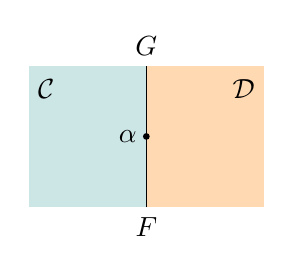
\begin{tikzpicture}
            \def\x{0};
            \def\xl{-1.5};
            \def\xr{1.5};


            \def \ya{0.8};
            \def \yb{1.7};
            \def \yc{2.6};
            \def \yt {2.3};

            \filldraw[fill=blue!50!green!20, draw=white] (\xl, \ya) rectangle (\x, \yc);
            \filldraw[fill=orange!30, draw=white] (\x, \ya) rectangle (\xr, \yc);

            \node[below] (a) at (\x, \ya) {$F$};
            \node(b) at (\x, \yb) {};
            \node [above] (c) at (\x, \yc) {$G$};

            \node(l)[right] at (\xl, \yt) {$\mathcal{C}$};
            \node(r)[left] at (\xr, \yt) {$\mathcal{D}$};


            \filldraw[black] (b) circle (1 pt);
            \node [left] at (b) {$\alpha$};

            \draw (a)  -- (c);

        \end{tikzpicture}
    \]

    这是一个\emph{字符串图(string diagram)}的示例。你从下到上、从左到右读取这样的图(想象一下$(x, y)$坐标系)。

    这个图的底部显示了从$\mathcal{C}$到$\mathcal{D}$的函子$F$。图的顶部显示了在同一对范畴之间的函子$G$。转变发生在中间,自然变换$\alpha$将$F$映射到$G$。

    在Haskell中,这个图表示为两个自函子之间的多态函数:
    \begin{haskell}
        alpha :: forall x. F x -> G x
    \end{haskell}

    到目前为止,使用这种新的视觉表示似乎并没有带来太多好处。但让我们将其应用于更有趣的东西:自然变换的垂直组合:
    \[
        \begin{tikzcd}[column sep=huge]
            \mathcal{C}
            \arrow[bend left=60]{rr}[name=U, label=above:$H$]{}
            \arrow[]{rr}[name=M, label={[xshift=15pt, yshift=-5pt]:$G$}]{}
            \arrow[bend right=60]{rr}[name=D, label=below:$F$]{}
            &&
            \mathcal{D}
            \arrow[shorten <=8pt, shorten >=8pt,Leftarrow, to path={(U) -- node[label=left:$\beta$] {} (M)}]{}
            \arrow[shorten <=8pt, shorten >=8pt,Leftarrow, to path={(M) -- node[label=left:$\alpha$] {} (D)}]{}
        \end{tikzcd}
    \]

    相应的字符串图显示了两个范畴以及它们之间由两个自然变换连接的三个函子。
    \[
        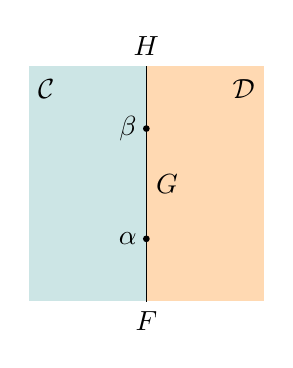
\begin{tikzpicture}
            \def\x{0};
            \def\xl{-1.5};
            \def\xr{1.5};


            \def \ya{0};
            \def \yb{0.8};
            \def \ybb{2.2};
            \def \yc{3};
            \def \yt {2.7};
            \def \ymid {1.5}

            \filldraw[fill=blue!50!green!20, draw=white] (\xl, \ya) rectangle (\x, \yc);
            \filldraw[fill=orange!30, draw=white] (\x, \ya) rectangle (\xr, \yc);

            \node[below] (a) at (\x, \ya) {$F$};
            \node(b) at (\x, \yb) {};
            \node(bb) at (\x, \ybb) {};
            \node [above] (c) at (\x, \yc) {$H$};
            \node(m)[right] at (\x, \ymid) {$G$};

            \node(l)[right] at (\xl, \yt) {$\mathcal{C}$};
            \node(r)[left] at (\xr, \yt) {$\mathcal{D}$};

            \filldraw[black] (b) circle (1 pt);
            \node [left] at (b) {$\alpha$};
            \filldraw[black] (bb) circle (1 pt);
            \node [left] at (bb) {$\beta$};

            \draw (a)  -- (c);

        \end{tikzpicture}
    \]
    如你所见,你可以通过从下到上扫描字符串图来重建原始图。

    在Haskell中,我们将处理三个自函子,以及$\hask{beta}$在$\hask{alpha}$之后的垂直组合:
    \begin{haskell}
        alpha :: forall x. F x -> G x
        beta  :: forall x. G x -> H x
    \end{haskell}
    使用常规函数组合来实现:
    \begin{haskell}
        beta_alpha :: forall x. F x -> H x
        beta_alpha = beta . alpha
    \end{haskell}

    让我们继续研究自然变换的水平组合:
    \[
        \begin{tikzcd}[column sep=huge]
            \mathcal{C}
            \arrow[bend left=50]{r}[name=U, label=above:$F'$]{}
            \arrow[bend right=50]{r}[name=D, label=below:$F$]{}
            &
            \mathcal{D}
            \arrow[bend left=50]{r}[name=U1, label=above:$G'$]{}
            \arrow[bend right=50]{r}[name=D1, label=below:$G$]{}
            &
            \mathcal{E}
            \arrow[shorten <=10pt,shorten >=10pt,Leftarrow,to path={(U) -- node[label=left:$\alpha$] {} (D)}]{}
            \arrow[shorten <=10pt,shorten >=10pt,Leftarrow,to path={(U1) -- node[label=left:$\beta$] {} (D1)}]{}
        \end{tikzcd}
    \]
    这次我们有三个范畴,因此我们将有三个区域。

    字符串图的底部对应于函子$G \circ F$(按此顺序)的组合。顶部对应于$G' \circ F'$。一个自然变换$\alpha$连接$F$到$F'$;另一个自然变换$\beta$连接$G$到$G'$。
    \[
        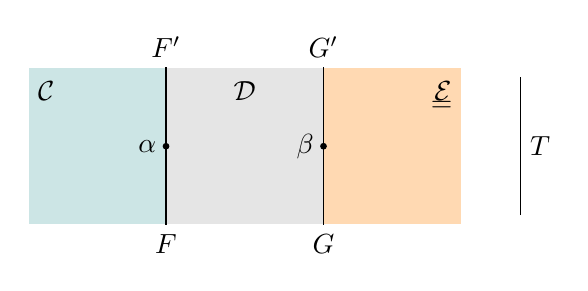
\begin{tikzpicture}
            \def\xl{-2.75};
            \def\xa{-1};
            \def\xc{0}
            \def\xb{1};
            \def\xr{2.75};


            \def \ya{0};
            \def \yb{1};
            \def \yc{2};
            \def \yt {1.7};

            \filldraw[fill=blue!50!green!20, draw=white] (\xl, \ya) rectangle (\xa, \yc);
            \filldraw[fill=black!10!white, draw=white] (\xa, \ya) rectangle (\xb, \yc);
            \filldraw[fill=orange!30, draw=white] (\xb, \ya) rectangle (\xr, \yc);

            \node[below] (a) at (\xa, \ya) {$F$};
            \node(b) at (\xa, \yb) {};
            \node [above] (c) at (\xa, \yc) {$F'$};

            \def\xd{3.5}
            \def\xe{2.5}
            \node(e) at (\xd, 0) {};
            \node(f) at (\xd, \yc) {};
            \node at (\xe, 1.5) {$=$};
            \draw (e) -- node[right] {$T$} (f);

            \node[below] (d) at (\xb, \ya) {$G$};
            \node(e) at (\xb, \yb) {};
            \node [above] (f) at (\xb, \yc) {$G'$};

            \node(l)[right] at (\xl, \yt) {$\mathcal{C}$};
            \node(r) at (\xc, \yt) {$\mathcal{D}$};
            \node(r)[left] at (\xr, \yt) {$\mathcal{E}$};


            \filldraw[black] (b) circle (1 pt);
            \node [left] at (b) {$\alpha$};
            \filldraw[black] (e) circle (1 pt);
            \node [left] at (e) {$\beta$};

            \draw (a)  -- (c);
            \draw (d)  -- (f);

        \end{tikzpicture}
    \]
    这个新的系统中,平行的垂直线对应于函子的组合。

    你可以认为自然变换的水平组合发生在图的中间的想象水平线上。但是,如果有人在绘制图时不够仔细,并且其中一个点比另一个点略高呢?事实证明,由于交换律,点的确切位置无关紧要。

    但首先,让我们说明whiskering:这是一个水平组合,其中一个自然变换是恒等的。我们可以这样绘制它:

    \[
        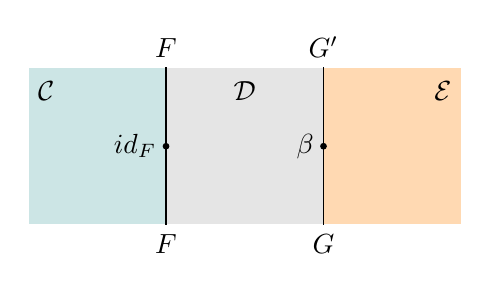
\begin{tikzpicture}
            \def\xl{-2.75};
            \def\xa{-1};
            \def\xc{0}
            \def\xb{1};
            \def\xr{2.75};


            \def \ya{0};
            \def \yb{1};
            \def \yc{2};
            \def \yt {1.7};

            \filldraw[fill=blue!50!green!20, draw=white] (\xl, \ya) rectangle (\xa, \yc);
            \filldraw[fill=black!10!white, draw=white] (\xa, \ya) rectangle (\xb, \yc);
            \filldraw[fill=orange!30, draw=white] (\xb, \ya) rectangle (\xr, \yc);

            \node[below] (a) at (\xa, \ya) {$F$};
            \node(b) at (\xa, \yb) {};
            \node [above] (c) at (\xa, \yc) {$F$};

            \node[below] (d) at (\xb, \ya) {$G$};
            \node(e) at (\xb, \yb) {};
            \filldraw[black] (e) circle (1 pt);
            \node [left] at (e) {$\beta$};

            \node [above] (f) at (\xb, \yc) {$G'$};

            \node(l)[right] at (\xl, \yt) {$\mathcal{C}$};
            \node(r) at (\xc, \yt) {$\mathcal{D}$};
            \node(r)[left] at (\xr, \yt) {$\mathcal{E}$};


            \filldraw[black] (b) circle (1 pt);
            \node [left] at (b) {$id_F$};

            \draw (a)  -- (c);
            \draw (d)  -- (f);

        \end{tikzpicture}
    \]
    但是,实际上,恒等可以插入到垂直线的任何位置,因此我们甚至不需要绘制它。以下图表示$\beta \circ F$的whiskering。
    \[
        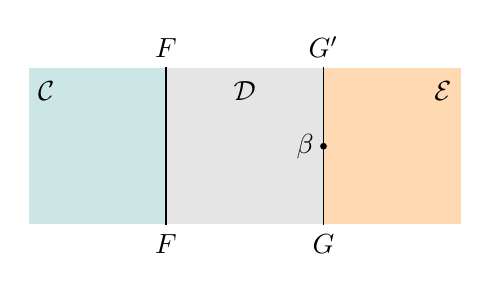
\begin{tikzpicture}
            \def\xl{-2.75};
            \def\xa{-1};
            \def\xc{0}
            \def\xb{1};
            \def\xr{2.75};


            \def \ya{0};
            \def \yb{1};
            \def \yc{2};
            \def \yt {1.7};

            \filldraw[fill=blue!50!green!20, draw=white] (\xl, \ya) rectangle (\xa, \yc);
            \filldraw[fill=black!10!white, draw=white] (\xa, \ya) rectangle (\xb, \yc);
            \filldraw[fill=orange!30, draw=white] (\xb, \ya) rectangle (\xr, \yc);

            \node[below] (a) at (\xa, \ya) {$F$};
            \node(b) at (\xa, \yb) {};
            \node [above] (c) at (\xa, \yc) {$F$};

            \node[below] (d) at (\xb, \ya) {$G$};
            \node(e) at (\xb, \yb) {};
            \node [above] (f) at (\xb, \yc) {$G'$};

            \node(l)[right] at (\xl, \yt) {$\mathcal{C}$};
            \node(r) at (\xc, \yt) {$\mathcal{D}$};
            \node(r)[left] at (\xr, \yt) {$\mathcal{E}$};

            \filldraw[black] (e) circle (1 pt);
            \node [left] at (e) {$\beta$};

            \draw (a)  -- (c);
            \draw (d)  -- (f);

        \end{tikzpicture}
    \]

    在Haskell中,当$\hask{beta}$是一个多态函数时:
    \begin{haskell}
        beta :: forall x. G x -> G' x
    \end{haskell}
    我们将这个图读作:
    \begin{haskell}
        beta_f :: forall x. G (F x) -> G' (F x)
        beta_f = beta
    \end{haskell}
    理解到类型检查器将实例化多态函数$\hask{beta}$为正确的类型。

    类似地,你可以轻松想象$G \circ \alpha$的图及其Haskell实现:
    \begin{haskell}
        g_alpha :: forall x. G (F x) -> G (F' x)
        g_alpha = fmap alpha
    \end{haskell}
    其中:
    \begin{haskell}
        alpha :: forall x. F x -> F' x
    \end{haskell}

    以下是对应于交换律的字符串图:
    \[
        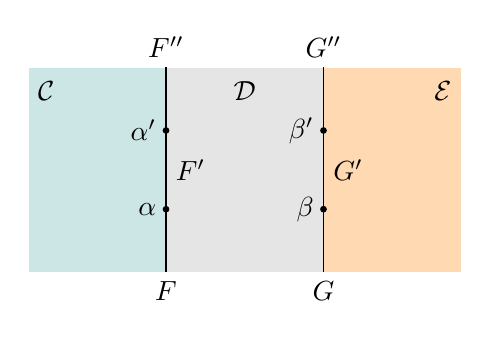
\begin{tikzpicture}
            \def\xl{-2.75};
            \def\xa{-1};
            \def\xc{0}
            \def\xb{1};
            \def\xr{2.75};


            \def \ya{0.2};
            \def \yb{1};
            \def \ybb{2}
            \def \yc{2.8};
            \def \yt {\yc -0.3};
            \def \ymid {1.5}

            \filldraw[fill=blue!50!green!20, draw=white] (\xl, \ya) rectangle (\xa, \yc);
            \filldraw[fill=black!10!white, draw=white] (\xa, \ya) rectangle (\xb, \yc);
            \filldraw[fill=orange!30, draw=white] (\xb, \ya) rectangle (\xr, \yc);

            \node[below] (a) at (\xa, \ya) {$F$};
            \node(b) at (\xa, \yb) {};
            \node [above] (c) at (\xa, \yc) {$F''$};
            \node [right] (ml) at (\xa, \ymid) {$F'$};

            \node[below] (d) at (\xb, \ya) {$G$};
            \node(e) at (\xb, \yb) {};
            \node [above] (f) at (\xb, \yc) {$G''$};
            \node [right] (ml) at (\xb, \ymid) {$G'$};

            \node(l)[right] at (\xl, \yt) {$\mathcal{C}$};
            \node(r) at (\xc, \yt) {$\mathcal{D}$};
            \node(r)[left] at (\xr, \yt) {$\mathcal{E}$};


            \filldraw[black] (b) circle (1 pt);
            \node [left] at (b) {$\alpha$};
            \filldraw[black] (e) circle (1 pt);
            \node [left] at (e) {$\beta$};

            \node(bb) at (\xa, \ybb) {};
            \node(ee) at (\xb, \ybb) {};

            \filldraw[black] (bb) circle (1 pt);
            \node [left] at (bb) {$\alpha'$};
            \filldraw[black] (ee) circle (1 pt);
            \node [left] at (ee) {$\beta'$};

            \draw (a)  -- (c);
            \draw (d)  -- (f);

        \end{tikzpicture}
    \]
    这个图故意模棱两可。我们应该先进行自然变换的垂直组合,然后再进行水平组合吗?还是应该水平组合$\beta \circ \alpha$和$\beta' \circ \alpha'$,然后再垂直组合结果?交换律告诉我们,这无关紧要:结果是相同的。

    现在尝试在此图中将一对自然变换替换为恒等变换。如果你替换$\alpha'$和$\beta'$,你会得到$\beta \circ \alpha$的水平组合。如果你用恒等自然变换替换$\alpha'$和$\beta$,并将$\beta'$重命名为$\beta$,你会得到一个图,其中$\alpha$相对于$\beta$向下移动,依此类推。

    \[
        \begin{tikzpicture}
            \def\xl{-2.75};
            \def\xa{-1};
            \def\xc{0}
            \def\xb{1};
            \def\xr{2.75};


            \def \ya{0.2};
            \def \yb{1};
            \def \ybb{2}
            \def \yc{2.8};
            \def \yt {\yc -0.3};
            \def \ymid {1.5}

            \filldraw[fill=blue!50!green!20, draw=white] (\xl, \ya) rectangle (\xa, \yc);
            \filldraw[fill=black!10!white, draw=white] (\xa, \ya) rectangle (\xb, \yc);
            \filldraw[fill=orange!30, draw=white] (\xb, \ya) rectangle (\xr, \yc);

            \node[below] (a) at (\xa, 0) {};
            \node(b) at (\xb, \yb) {};
            \node [above] (c) at (\xa, \yc) {$F'$};

            \node[below] (d) at (\xb, \ya) {$G$};
            \node(e) at (\xb, \yb) {};
            \filldraw[black] (e) circle (1 pt);
            \node [left] at (e) {$\beta$};

            \draw (a)  -- (c);
            \draw (d)  -- (f);

        \end{tikzpicture}
    \]
    交换律告诉我们,所有这些图都是相等的。我们可以像珠子穿在线上一样自由滑动自然变换。

    \subsection{String diagrams for the monad\text{(单子的字符串图)}}

    一个单子定义为一个配备了两个自然变换的自函子,如下图所示:

    \[
        \begin{tikzcd}[column sep=huge]
            \mathcal{C}
            \arrow[bend left=50]{r}[name=U, label=above:$T$]{}
            \arrow[bend right=50]{r}[name=D, label=below:$\text{Id}$]{}
            &
            \mathcal{C}
            \arrow[shorten <=10pt,shorten >=10pt,Leftarrow,to path={(U) -- node[label=left:$\eta$] {} (D)}]{}
        \end{tikzcd}
        \hspace{20pt}
        \begin{tikzcd}[column sep=huge]
            \mathcal{C}
            \arrow[bend left=50]{r}[name=U, label=above:$T$]{}
            \arrow[bend right=50]{r}[name=D, label=below:$T \circ T$]{}
            &
            \mathcal{C}
            \arrow[shorten <=10pt,shorten >=10pt,Leftarrow,to path={(U) -- node[label=left:$\mu$] {} (D)}]{}
        \end{tikzcd}
    \]

    由于我们只处理一个范畴,当将这些图转换为字符串图时,我们可以省略范畴的命名(和着色),只绘制字符串。

    \[
        \begin{tikzpicture}

            \def \xleft{-2}

            \def\xa{0};
            \def\xb{0.7};
            \def\xc{\xb * 2};

            \def \ya{0};
            \def \yb{1};
            \def \yc{2};

            \node(a) at (\xleft, \ya) {};
            \node(b) at (\xleft, \yb) {}; % middle
            \node(c) at (\xleft, \yc) {};

            \draw[dashed] (a) -- node[right] {$\text{Id}$} (b);
            \draw (b) -- node[right] {$T$} (c);


            \node(d) at (\xa, \ya) {};
            \node(e) at (\xc, \ya) {};
            \node(f) at (\xb, \yb) {}; % middle
            \node(g) at (\xb, \yc) {}; % top


            \filldraw[black] (b) circle (1 pt);
            \node [left] at (b) {$\eta$};

            \draw (d) to [out=90, in=180]  node[left] {$T$}(f);
            \draw (e) to [out=90, in=0]  node[right] {$T$} (f);

            \draw (f) -- node[right] {$T$} (g);

            \filldraw[black] (f) circle (1 pt);
            \node [below] at (f) {$\mu$};

        \end{tikzpicture}
    \]
    在第一个图中,通常会跳过表示恒等函子的虚线。$\eta$点可以自由地将$T$线注入到图中。两个$T$线可以通过$\mu$点连接。

    字符串图在表达单子律时特别有用。例如,我们有左恒等律:
    \[ \mu \circ (\eta \circ T) = id \]
    这可以用一个交换图来表示:
    \[
        \begin{tikzcd}
            \text{Id} \circ T
            \arrow[rr, "\eta \circ T"]
            \arrow[rrd, "id"']
            & & T \circ T
            \arrow[d, "\mu"]
            \\
            && T
        \end{tikzcd}
    \]
    相应的字符串图表示通过这个图的两条路径的相等性:

    \[
        \begin{tikzpicture}
            \def\xa{0};
            \def\xb{0.7};
            \def\xc{\xb * 2};

            \def \ya{0.8};
            \def \yb{1.7};
            \def \yc{2.6};

            \node(a) at (\xa, \ya) {};
            \node(b) at (\xb, \yb) {};
            \node(c) at (\xc, 0) {};
            \node(d) at (\xb, \yc) {};
            \filldraw[black] (a) circle (1 pt);
            \node [below] at (a) {$\eta$};
            \filldraw[black] (b) circle (1 pt);
            \node [below] at (b) {$\mu$};
            \draw (a) to [out=90, in=180]  node[left] {$T$}(b);
            \draw (c) to [out=90, in=0]  node[right] {$T$} (b);
            \draw (b) -- node[right] {$T$} (d);

            \def\xd{3.5}
            \def\xe{2.5}
            \node(e) at (\xd, 0) {};
            \node(f) at (\xd, \yc) {};
            \node at (\xe, 1.5) {$=$};
            \draw (e) -- node[right] {$T$} (f);
        \end{tikzpicture}
    \]
    你可以将此等式视为通过拉扯上下字符串,使$\eta$附属物缩回到直线中。

    同样有一个对称的右恒等律:
    \[
        \begin{tikzpicture}
            \def\xa{0};
            \def\xb{0.7};
            \def\xc{\xb * 2};

            \def \ya{0.8};
            \def \yb{1.7};
            \def \yc{2.6};

            \node(a) at (\xa, 0) {};
            \node(b) at (\xb, \yb) {};
            \node(c) at (\xc, \ya) {};
            \node(d) at (\xb, \yc) {};
            \filldraw[black] (b) circle (1 pt);
            \node [below] at (c) {$\eta$};
            \filldraw[black] (c) circle (1 pt);
            \node [below] at (b) {$\mu$};
            \draw (a) to [out=90, in=180]  node[left] {$T$}(b);
            \draw (c) to [out=90, in=0]  node[right] {$T$} (b);
            \draw (b) -- node[right] {$T$} (d);

            \def\xd{3.5}
            \def\xe{2.5}
            \node(e) at (\xd, 0) {};
            \node(f) at (\xd, \yc) {};
            \node at (\xe, 1.5) {$=$};
            \draw (e) -- node[right] {$T$} (f);
        \end{tikzpicture}
    \]

    最后,这是关联律的字符串图表示:
    \[
        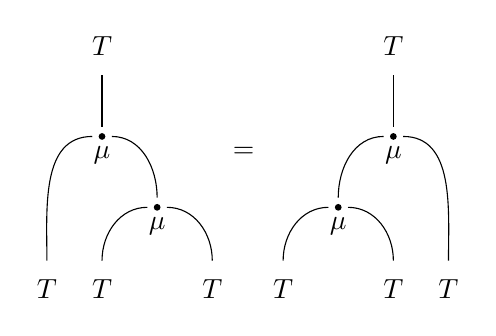
\begin{tikzpicture}
            \def\delta{0.7}
            \def\xa{0};
            \def\xb{\delta};
            \def\xc{\delta * 2};
            \def\xd{\delta * 3};

            \def \ya{0.8};
            \def \yb{1.7};
            \def \yc{2.6};

            \node(a) at (\xa, 0) {};
            \node(b) at (\xb, \yb) {};
            \node(c) at (\xc, \ya) {};
            \node(d) at (\xb, \yc) {};
            \node(e) at (\xb, 0) {};
            \node(f) at (\xd, 0) {};
            \filldraw[black] (b) circle (1 pt);
            \filldraw[black] (c) circle (1 pt);
            \node [below] at (b) {$\mu$};
            \draw (a) to [out=90, in=180]  node[left] {}(b);
            \draw (c) to [out=90, in=0]  node[right] {} (b);
            \draw (b) -- node[right] {} (d);
            \draw (e) to [out=90, in=180]  node[left] {}(c);
            \draw (f) to [out=90, in=0]  node[right] {}(c);
            \node [below] at (c) {$\mu$};
            \node [below] at (a) {$T$};
            \node [above] at (d) {$T$};
            \node [below] at (e) {$T$};
            \node [below] at (f) {$T$};

            \def\xe{2.5}
            \node at (\xe, 1.5) {$=$};

            \def\off{3}
            \def\xa{\off + \delta * 0};
            \def\xb{\off + \delta * 1};
            \def\xc{\off + \delta * 2};
            \def\xd{\off + \delta * 3};

            \node(a) at (\xa, 0) {};
            \node(b) at (\xc, 0) {};
            \node(c) at (\xd, 0) {};
            \node(d) at (\xb, \ya) {};
            \node(e) at (\xc, \yb) {};
            \node(f) at (\xc, \yc) {};
            \filldraw[black] (d) circle (1 pt);
            \filldraw[black] (e) circle (1 pt);
            \node [below] at (d) {$\mu$};
            \draw (a) to [out=90, in=180]  node[left] {}(d);
            \draw (b) to [out=90, in=0]  node[right] {} (d);
            \draw (e) -- node[right] {} (f);
            \draw (d) to [out=90, in=180]  node[left] {}(e);
            \draw (c) to [out=90, in=0]  node[right] {}(e);
            \node [below] at (e) {$\mu$};
            \node [below] at (a) {$T$};
            \node [below] at (b) {$T$};
            \node [below] at (c) {$T$};
            \node [above] at (f) {$T$};
        \end{tikzpicture}
    \]

    \subsection{String diagrams for the adjunction\text{(伴随函子的字符串图)}}

    正如我们之前讨论的,伴随函子是两个函子之间的关系,$L \colon \mathcal{D} \to \mathcal{C}$和$R \colon \mathcal{C} \to \mathcal{D}$。它可以通过一对自然变换来定义,伴随单元$\eta$和伴随余单元$\varepsilon$,它们满足三角恒等式。

    伴随单元可以通过一个“杯”形图来说明:

    \[
        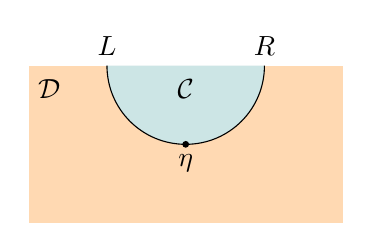
\begin{tikzpicture}

            \def \xrightmost {2}
            \def \xright         {1}
            \def \xmid          {0}
            \def \xleft           {-\xright}
            \def \xleftmost   {-\xrightmost}

            \def \ybot           {0}
            \def \ymid          {1}
            \def \ytop           {2}
            \def \ylabel        {\ytop - 0.3}

% functor labels
            \node [above] at (\xleft, \ytop)   {$L$};
            \node [above] at (\xright, \ytop) {$R$};
% background
            \filldraw[fill=orange!30, draw=white] (\xleftmost, \ytop) rectangle (\xrightmost, \ybot);
% cup
            \draw [fill=blue!50!green!20] (\xleft, \ytop) to [out=-90, in=180] (\xmid, \ymid) to [out=0, in=-90] (\xright, \ytop);
% natural transformation
            \filldraw [black] (\xmid, \ymid) circle (1 pt);
            \node [below] at (\xmid, \ymid) {$\eta$};
% category labels
            \node           at (\xmid, \ylabel)        {$\mathcal{C}$};
            \node [right] at (\xleftmost, \ylabel) {$\mathcal{D}$};

        \end{tikzpicture}
    \]
    图底部的恒等函子从图中省略了。$\eta$点将其下方的恒等函子转变为其上方的组合$R \circ L$。

    类似地,伴随余单元可以通过一个“帽”形字符串图来可视化,顶部的隐含恒等函子:

    \[
        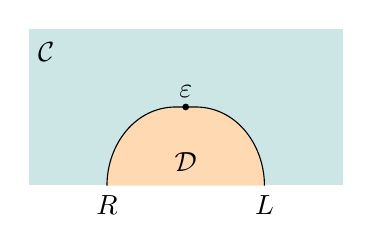
\begin{tikzpicture}
            \def\xleft{0};
            \def\xmid{1};
            \def\xright{\xmid * 2};

            \def \ybot{0};
            \def \ymid{1};
            \def \ytop{2 * \ymid};
            \def \yt{2 * \ymid - 0.3};

            \node [below] (a) at (\xleft, \ybot) {$R$};
            \node(b) at (\xmid, \ymid) {};
            \node[below] (c) at (\xright, \ybot) {$L$};

            \filldraw[fill=blue!50!green!20, draw=white] (\xleft-1, \ytop) rectangle (\xright+1, \ybot);


            \draw [fill=orange!30] (a.north) to [out=90, in=180] (b.west) -- (b.east) to [out=0, in=90] (c.north);

            \filldraw[black] (b) circle (1 pt);
            \node [above] at (b) {$\varepsilon$};

            \node(l)[right] at (\xleft-1, \yt) {$\mathcal{C}$};
            \node(r) at (\xmid, \ybot + 0.3) {$\mathcal{D}$};

        \end{tikzpicture}
    \]

    三角恒等式可以使用字符串图轻松表达。它们也很直观,因为你可以想象从两边拉动字符串以拉直曲线。

    例如,这是第一个三角恒等式,有时称为\index{zigzag identity}\emph{之字形恒等式}:

    \[
        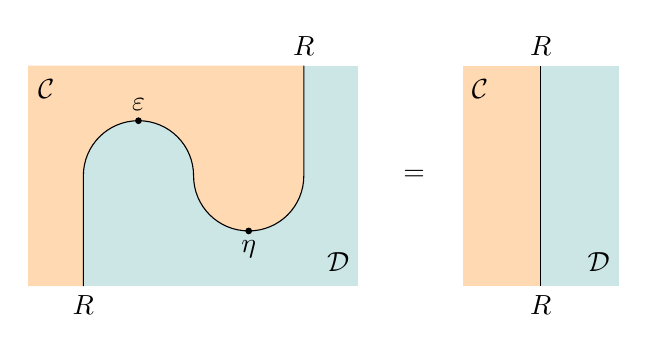
\begin{tikzpicture}
            \def \dx {0.7}
            \def \dy {0.7}

            \def \xa{-3 * \dx};
            \def \xb{-2 * \dx};
            \def \xc{-1 * \dx};
            \def \xd{0};
            \def \xe{1 * \dx};
            \def \xf{2 * \dx};
            \def \xg{3 * \dx};

            \def \ya{0};
            \def \yb{1 * \dy};
            \def \yc{2 * \dy};
            \def \yd{3 * \dy};
            \def \ye{4 * \dy};

            \node [below] at (\xb, \ya) {$R$};
            \node [right] at (\xd, \yc) {$L$};
            \node [above] at (\xf, \ye) {$R$};
% background
            \filldraw[fill=blue!50!green!20, draw=white] (\xa, \ye) rectangle (\xg, \ya);
% fill shape
            \path [fill=orange!30] (\xa, \ya) to (\xb, \ya) to (\xb, \yc) to [out=90, in=180]  (\xc, \yd) to  [out=0, in=90] (\xd, \yc) to [out=-90, in=180] (\xe, \yb) to [out=0, in=-90] (\xf, \yc) to (\xf, \ye) to (\xa, \ye);

            \draw (\xb, \ya) to (\xb, \yc) to [out=90, in=180]  (\xc, \yd) to  [out=0, in=90] (\xd, \yc) to [out=-90, in=180] (\xe, \yb) to [out=0, in=-90] (\xf, \yc) to (\xf, \ye);

            \filldraw[black] (\xc, \yd) circle (1 pt);
            \node [above] at (\xc, \yd) {$\varepsilon$};

            \filldraw[black] (\xe, \yb) circle (1 pt);
            \node [below] at (\xe, \yb) {$\eta$};

            \node[right] at (\xa, \ye - 0.3) {$\mathcal{C}$};
            \node[left] at (\xg, \ya + 0.3) {$\mathcal{D}$};

% right diagram

            \node (eq) at (4 * \dy, \yc) {$=$};
            \def \xh {6.3 * \dx}

            \filldraw[fill=orange!30, draw=white] (\xh - 1, \ye) rectangle (\xh, \ya);
            \filldraw[fill=blue!50!green!20, draw=white] (\xh, \ye) rectangle (\xh + 1, \ya);

            \draw (\xh, \ye) -- (\xh, \ya);

            \node[below] (bb) at (\xh, \ya) { $R$ };
            \node[above] (bt) at (\xh, \ye) { $R$ };

            \node(l)[right] at (\xh - 1, \ye - 0.3) {$\mathcal{C}$};
            \node(r)[left] at (\xh + 1, \ya + 0.3) {$\mathcal{D}$};

        \end{tikzpicture}
    \]
    从下到上读取左图,会得到一系列映射:

    \[  Id_{\mathcal{D}} \circ R \xrightarrow{\eta \circ R} R \circ L \circ R \xrightarrow{R \circ \varepsilon} R \circ Id_{\mathcal{C}}  \]
    这必须等于右侧,它可以被解释为$\hask{R}$上的(隐形)恒等自然变换。

    在$\hask{R}$是自函子的情况下,我们可以将第一个图直接翻译为Haskell。$\hask{R}$对伴随单元$\eta$的whiskering导致多态函数$\hask{unit}$在$\hask{R x}$上实例化。伴随余单元$\varepsilon$的whiskering导致$\hask{counit}$由函子$\hask{R}$提升。垂直组合翻译为函数组合:
    \begin{haskell}
        triangle :: forall x. R x -> R x
        triangle = fmap counit . unit
    \end{haskell}

    \begin{exercise}
        Draw the string diagrams for the second triangle identity and translate them to Haskell.
    \end{exercise}

    \section{Monads from Adjunctions(从伴随构造单子)}

    你可能已经注意到,$\eta$这个符号既用于伴随单元,也用于单子单元。这\emph{不是}巧合。

    乍一看,这似乎是将苹果与橙子进行比较:伴随是由两个类别之间的两个函子定义的,而单子是由在一个类别上操作的一个自函子定义的。然而,两个反向函子的组合是一个自函子,并且伴随的单元将恒等自函子映射到自函子$R \circ L$。

    对比这个图:

    \[
        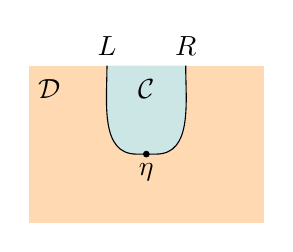
\begin{tikzpicture}
            \def\xleft{0.5};
            \def\xmid{1};
            \def\xright{1.5};

            \def \ybot{0};
            \def \ymid{1};
            \def \ytop{2 * \ymid};
            \def \yt{2 * \ymid - 0.3};

            \node [above] (a) at (\xleft, \ytop) {$L$};
            \node(b) [below] at (\xmid, \ymid) {};
            \node[above] (c) at (\xright, \ytop) {$R$};

            \filldraw[fill=orange!30, draw=white] (\xleft-1, \ytop) rectangle (\xright+1, \ybot);

            \draw [fill=blue!50!green!20] (a.south) to [out=-90, in=180] (b.west) -- (b.east) to [out=0, in=-90] (c.south);
            \filldraw[black] (b) circle (1 pt);
            \node [below] at (b) {$\eta$};

            \node(l)[right] at (\xleft-1, \yt) {$\mathcal{D}$};
            \node(r) at (\xmid, \yt) {$\mathcal{C}$};

        \end{tikzpicture}
    \]
    与定义单子单元的这个图:

    \[
        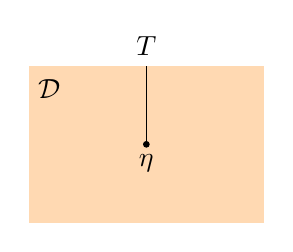
\begin{tikzpicture}
            \def\xleft{0.5};
            \def\xmid{1};
            \def\xright{1.5};

            \def \ybot{0};
            \def \ymid{1};
            \def \ytop{2 * \ymid};
            \def \yt{2 * \ymid - 0.3};

            \node(b) [above] at (\xmid, \ytop) {$T$};

            \filldraw[fill=orange!30, draw=white] (\xleft-1, \ytop) rectangle (\xright+1, \ybot);

            \draw (\xmid, \ymid) -- (\xmid, \ytop);

            \filldraw[black] (\xmid, \ymid) circle (1 pt);
            \node [below] at (\xmid, \ymid) {$\eta$};

            \node(l)[right] at (\xleft-1, \yt) {$\mathcal{D}$};

        \end{tikzpicture}
    \]

    事实证明,对于任何伴随$L \dashv R$,自函子$T = R \circ L$是一个单子,其乘法$\mu$由以下图定义:

    \[
        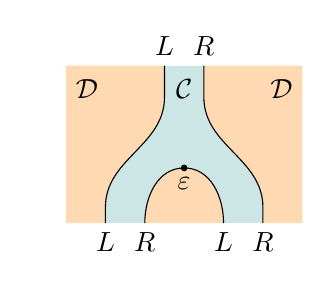
\begin{tikzpicture}
            \def \xmid          {0};
            \def \xr               {0.5};
            \def \xrr             {1}
            \def \xrm            {0.25}
            \def \xrightmost {1.5}
            \def \xl {-\xr}
            \def \xll {-\xrr}
            \def \xlm {-\xrm}
            \def \xleftmost {-\xrightmost}

            \def \ybot           {0};
            \def \ymidbot     {0.20};
            \def \yeps          {0.7};
            \def \ymid          {1};
            \def \ymidtop     {1.60}
            \def \ytop           {2};
            \def \ylabel        {\ytop - 0.3};
% functors
            \node [above] at (\xlm, \ytop)  {$L$};
            \node [above] at (\xrm, \ytop) {$R$};
            \node [below] at (\xll, \ybot) {$L$};
            \node [below] at (\xl, \ybot) {$R$};
            \node [below] at (\xr, \ybot) {$L$};
            \node [below] at (\xrr, \ybot) {$R$};

            \filldraw[fill=blue!50!green!20, draw=white, draw=white] (\xleftmost, \ytop) rectangle (\xrightmost, \ybot);

% left area
            \path [fill=orange!30] (\xleftmost, \ybot) to  (\xll, \ybot) to (\xll, \ymidbot) [out=90, in=-90] to (\xlm, \ymidtop) to  (\xlm, \ytop) to [out=180, in=180] (\xleftmost, \ytop);
% right area
            \path [fill=orange!30] (\xrightmost, \ybot) to (\xrr, \ybot) to (\xrr, \ymidbot) [out=90, in=-90] to (\xrm, \ymidtop) to (\xrm, \ytop) to [out=0, in=180]  (\xrightmost, \ytop);
% cap
            \draw [fill=orange!30] (\xl, \ybot) to [out=90, in=180] (\xmid, \yeps) to [out=0, in=90] (\xr, \ybot);
% left curve
            \draw (\xll, \ybot) to (\xll, \ymidbot) [out=90, in=-90] to (\xlm, \ymidtop) to  (\xlm, \ytop);
% right curve
            \draw (\xrr, \ybot) to (\xrr, \ymidbot) [out=90, in=-90] to (\xrm, \ymidtop) to (\xrm, \ytop);
% epsilon
            \filldraw [black] (\xmid, \yeps) circle (1 pt);
            \node [below] at (\xmid, \yeps) {$\varepsilon$};
% categories
            \node [right] at (\xleftmost, \ylabel) {$\mathcal{D}$};
            \node           at (\xmid, \ylabel)        {$\mathcal{C}$};
            \node [left]   at (\xrightmost, \ylabel) {$\mathcal{D}$};

        \end{tikzpicture}
    \]
    从下到上读取这个图,我们得到以下变换(想象将其水平切片在点处):
    \[  R \circ L \circ R \circ L \xrightarrow{R \circ \varepsilon \circ L} R \circ L  \]
    与单子的$\mu$定义比较:

    \[
        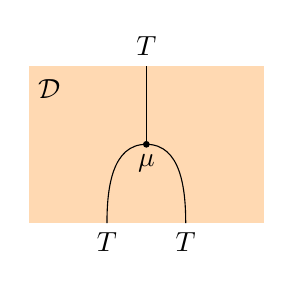
\begin{tikzpicture}
            \def \xmid          {0};
            \def \xr               {0.5};
            \def \xrightmost {1.5};
            \def \xl {-\xr};
            \def \xleftmost {-\xrightmost};

            \def \ybot           {0};
            \def \ymid          {1};
            \def \ytop           {2};
            \def \ylabel        {\ytop - 0.3};

            \node [above] at (\xmid, \ytop) {$T$};
            \node [below] at (\xl, \ybot)      {$T$};
            \node [below] at (\xr, \ybot)      {$T$};

            \filldraw[fill=orange!30, draw=white] (\xleftmost, \ytop) rectangle (\xrightmost, \ybot);
% cap
            \draw (\xl, \ybot) to [out=90, in=180] (\xmid, \ymid) to [out=0, in=90] (\xr, \ybot);
            \draw (\xmid, \ymid) to (\xmid, \ytop);

            \filldraw [black] (\xmid, \ymid) circle (1 pt);
            \node [below] at (\xmid, \ymid) {$\mu$};

            \node [right] at (\xleftmost, \ylabel) {$\mathcal{D}$};

        \end{tikzpicture}
    \]
    我们得到了单子$R \circ L$的$\mu$定义,其为$\varepsilon$的双whiskering:
    \[ \mu = R \circ \varepsilon \circ L \]

    以$\varepsilon$为基础定义$\mu$的字符串图可以始终转换为Haskell代码。单子的乘法,或称为\hask{join},变为:
    \begin{haskell}
        join :: forall x. T (T x) -> T x
        join = fmap counit
    \end{haskell}
    其中\hask{fmap}对应于由自函子\hask{T}(定义为组合$R \circ L$)提升的函数。注意在这种情况下,$\cat D$是Haskell类型和函数的范畴,但$\cat C$可以是一个外部范畴。

    为了完成这个图,我们可以使用字符串图,通过三角等式推导出单子定律。诀窍是将单子定律中的所有字符串替换为成对的平行字符串,然后根据规则重新排列它们。

    总结来说,每个具有单元$\eta$和余单元$\varepsilon$的伴随$L \dashv R$定义了一个单子$(R \circ L, \eta, R \circ \varepsilon \circ L)$。

    稍后我们将看到,反之,另一个组合$L \circ R$定义了一个余单子。

    \begin{exercise}
        Draw string diagrams to illustrate monadic laws (unit and associativity) for the monad derived from an adjunction.
        (请绘制字符串图,来说明从伴随推导出的单子的单子定律(单位元和结合律))
    \end{exercise}

    \section{Examples of Monads from Adjunctions(从伴随推导出的单子示例)}

    我们将通过几个示例来展示从伴随生成的一些在编程中使用的单子。在讨论单子转换器时,我们将进一步展开这些示例。

    大多数示例涉及将函子离开Haskell类型和函数的范畴,尽管生成单子的循环最终成为自函子。这就是为什么在Haskell中经常无法表达这样的伴随的原因。

    为了进一步复杂化,存在很多与显式命名数据构造函数相关的簿记工作,这是类型推断所必需的。这有时可能会掩盖底层公式的简单性。

    \subsection{Free monoid and the list monad(自由幺半群与列表单子)}
    列表单子由我们之前见过的自由幺半群伴随生成。该伴随的单元$\eta_X \colon X \to U (F X)$将集合$X$的元素注入为自由幺半群$F X$的生成元,之后$U$提取底层集合。

    在Haskell中,我们将自由幺半群表示为列表类型,其生成元是单元素列表。$\eta_X$将$X$的元素映射为这些单元素列表:
    \begin{haskell}
        return x = [x]
    \end{haskell}
    为了实现余单元$\varepsilon_M \colon F (U M) \to M$,我们取一个幺半群$M$,忘记其乘法,并使用其元素集作为新的自由幺半群的生成元。余单元在$M$上的分量是从自由幺半群返回到$M$的幺半群同态,或者在Haskell中是\hask{[m]->m}。事实证明,这种幺半群同态是一个特殊的归纳同态。

    首先,回顾一下Haskell实现的一般列表归纳同态:
    \begin{haskell}
        foldMap :: Monoid m => (a -> m) -> ([a] -> m)
        foldMap f = foldr mappend mempty . fmap f
    \end{haskell}
    在这里,我们将\hask{(a -> m)}解释为从\hask{a}到幺半群\hask{m}底层集合的常规函数。结果被解释为从\hask{a}生成的自由幺半群(即\hask{a}的列表)到\hask{m}的\emph{幺半群同态}。这只是伴随的一个方向:
    \[ \Set (a, U m) \cong \Cat{Mon} (F a, m) \]

    为了获得作为幺半群同态的余单元\hask{[m]->m},我们将\hask{foldMap}应用于恒等式。结果是\hask{(foldMap id)},或者在\hask{foldr}的术语中:
    \begin{haskell}
        epsilon = foldr mappend mempty
    \end{haskell}
    这是一个幺半群同态,因为它将空列表映射到幺半群单元,并将连接映射到幺半群乘积。

    单子乘法或\hask{join}由余单元的whiskering给出:
    \[ \mu = U \circ \varepsilon \circ F \]
    你可以很容易地说服自己,左whiskering在这里并没有做太多,因为它只是通过遗忘函子提升了一个幺半群同态(它保留了函数而忘记了其保持结构的特殊属性)。

    右边的$F$的whiskering更有趣。这意味着分量$\mu_X$对应于$\varepsilon$在$F X$上的分量,这是从集合$X$生成的自由幺半群。这个自由幺半群由以下定义:
    \begin{haskell}
        mempty = []
        mappend = (++)
    \end{haskell}
    这给出了\hask{join}的定义:
    \begin{haskell}
        join = foldr (++) []
    \end{haskell}
    正如预期的那样,这与\hask{concat}相同:在列表单子中,乘法是连接。

    \subsection{The currying adjunction and the state monad(柯里化伴随与状态单子)}

    状态单子由我们用来定义指数对象的柯里化伴随生成。左函子由与某个固定对象$s$的乘积定义:
    \[ L_s a = a \times s \]
    例如,我们可以将其实现为Haskell类型:
    \begin{haskell}
        newtype L s a = L (a, s)
    \end{haskell}
    右函子是指数化,以同一个对象$s$为参数化:
    \[ R_s c = c^s \]
    在Haskell中,它是一个薄封装的函数类型:
    \begin{haskell}
        newtype R s c = R (s -> c)
    \end{haskell}

    单子由这两个函子的组合给出。在对象上:
    \[(R_s \circ L_s) a = (a \times s)^s \]
    在Haskell中我们会写成:
    \begin{haskell}
        newtype St s a = St (R s (L s a))
    \end{haskell}
    如果你展开这个定义,很容易在其中识别出\hask{State}函子:
    \begin{haskell}
        newtype State s a = State (s -> (a, s))
    \end{haskell}

    伴随$L_s \dashv R_s$的单元是一个映射:
    \[ \eta_a \colon a \to (a \times s)^s \]
    它可以在Haskell中实现为:
    \begin{haskell}
        unit :: a -> R s (L s a)
        unit a = R (\s -> L (a, s))
    \end{haskell}
    你可能已经在其中识别出状态单子的\hask{return}的一个薄薄版本:
    \begin{haskell}
        return :: a -> State s a
        return a = State (\s -> (a, s))
    \end{haskell}

    这里是伴随在$c$上的余单元的分量:
    \[ \varepsilon_c \colon c^s \times s \to c \]
    它可以在Haskell中实现为:
    \begin{haskell}
        counit :: L s (R s a) -> a
        counit (L ((R f), s))= f s
    \end{haskell}
    在剥离了数据构造器后,它等价于\hask{apply},或\hask{runState}的非柯里化版本。

    单子乘法$\mu$由$\varepsilon$的whiskering从两侧给出:
    \[ \mu = R_s \circ \varepsilon \circ L_s \]
    以下是其转换为Haskell的版本:
    \begin{haskell}
        mu :: R s (L s (R s (L s a))) -> R s (L s a)
        mu = fmap counit
    \end{haskell}
    右边的whiskering除了选择自然变换的分量之外什么也不做。这是Haskell的类型推断引擎自动完成的。左边的whiskering是通过提升自然变换的分量完成的。同样,类型推断会选择正确的\hask{fmap}实现——这里它等同于前置组合。

    与\hask{join}的实现进行比较:
    \begin{haskell}
        join :: State s (State s a) -> State s a
        join mma = State (fmap (uncurry runState) (runState mma))
    \end{haskell}
    注意\hask{runState}的双重使用:
    \begin{haskell}
        runState :: State s a -> s -> (a, s)
        runState (State h) s = h s
    \end{haskell}
    当它被非柯里化时,它的类型签名变为:
    \begin{haskell}
        uncurry runState :: (State s a, s) -> (a, s)
    \end{haskell}
    这与\hask{counit}的类型签名相同。

    当部分应用时,\hask{runState}只是剥离了数据构造器,暴露了底层函数类型:
    \begin{haskell}
        runState st :: s -> (a, s)
    \end{haskell}

    \subsection{M-sets and the writer monad(M-集与writer单子)}

    writer单子:
    \begin{haskell}
        newtype Writer m a = Writer (a, m)
    \end{haskell}
    由一个幺半群\hask{m}参数化。该幺半群用于累积日志条目。我们将使用的伴随涉及该幺半群的M-集范畴。

    一个\index{M-set}M-集是一个集合$S$,我们在其上定义幺半群$M$的作用。这样的作用是一个映射:
    \[a \colon M \times S \to S \]
    我们经常使用作用的柯里化版本,幺半群元素位于下标位置。因此$a_m$成为$S \to S$的函数。

    这个映射必须满足一些约束。幺半群单位$1$的作用不能改变集合,因此它必须是恒等函数:
    \[ a_1 = id_S \]
    并且两个连续的作用必须组合成其幺半群乘积的作用:
    \[ a_{m_1} \circ a_{m_2} = a_{m_1 \cdot m_2} \]
    这种乘法顺序的选择定义了所谓的\emph{左作用}。(右作用将右侧的两个幺半群元素交换。)

    M-集形成一个范畴$\mathbf{MSet}$。对象是对$(S, a\colon M\times S \to S)$,箭头是\index{equivariant map}\emph{协变映射},即保持作用的集合之间的函数。

    函数$f \colon S \to R$是从$(S, a)$到$(R, b)$的\emph{协变}映射,如果以下图对每个$m \in M$都交换:

    \[
        \begin{tikzcd}
            S
            \arrow[r, "f"]
            \arrow[d, "a_m"]
            & R
            \arrow[d, "b_m"]
            \\
            S
            \arrow[r, "f"]
            & R
        \end{tikzcd}
    \]
    换句话说,我们可以先进行作用$a_m$,然后映射集合;或者先映射集合,然后进行相应的作用$b_m$,效果是相同的。

    从$\mathbf{MSet}$到$\mathbf{Set}$有一个遗忘函子$U$,它将集合$S$分配给对$(S, a)$,从而遗忘了作用。

    与之对应的是一个自由函子$F$。它在集合$S$上的作用产生一个M-集。它是一个$S$和$M$的笛卡尔积的集合,其中$M$被视为元素的集合(换句话说,遗忘函子作用在幺半群上的结果)。这个M-集的元素是对$(x \in S, m \in M)$,自由作用由以下定义:
    \[ \phi_n \colon (x, m) \mapsto (x, n \cdot m) \]
    保持元素$x$不变,仅乘以$m$分量。

    为了表明$F$是$U$的左伴随,我们必须构造以下自然同构:
    \[ \mathbf{MSet}( F S, Q) \cong \mathbf{Set}(S, U Q) \]
    对于任何集合$S$和任何M-集$Q$。如果我们将$Q$表示为对$(R, b)$,则伴随右侧的元素是普通函数$u \colon S \to R$。我们可以使用此函数在左侧构造一个协变映射。

    这里的技巧是注意到这样的协变映射$f \colon F S \to Q$由其在形式$(x, 1) \in F S$的元素上的作用完全确定,其中$1$是幺半群单位。

    事实上,从协变条件可以得出:

    \[
        \begin{tikzcd}
        (x, 1)
            \arrow[r, mapsto, "f"]
            \arrow[d, mapsto, "\phi_m"]
            & r
            \arrow[d, mapsto, "b_m"]
            \\
            (x, m \cdot 1)
            \arrow[r, mapsto, "f"]
            & r'
        \end{tikzcd}
    \]
    或者:
    \[ f( \phi_m (x, 1)) = f (x, m) = b_m ( f (x, 1)) \]
    因此,每个函数$u \colon S \to R$唯一地定义了从$F S$到$Q$的协变映射$f \colon F S \to Q$,给出:
    \[ f (x, m) = b_m (u x) \]

    这个伴随的单元$\eta_S \colon S \to U (F S)$将元素$x$映射为对$(x, 1)$。将此与writer单子的\hask{return}定义进行比较:
    \begin{haskell}
        return a = Writer (a, mempty)
    \end{haskell}

    余单元由一个协变映射给出:
    \[ \varepsilon_Q \colon F (U Q) \to Q \]

    左侧是通过取$Q$的底层集合并将其与$M$的底层集合取积构造的M-集。$Q$的原始作用被遗忘并由自由作用取代。余单元的显然选择是:
    \[ \varepsilon_Q \colon (x, m) \mapsto a_m x \]
    其中$x$是(底层集合的)$Q$的一个元素,而$a$是在$Q$中定义的作用。

    单子乘法$\mu$由余单元的whiskering给出。
    \[ \mu = U \circ \varepsilon \circ F \]
    这意味着在$\varepsilon_Q$的定义中用自由作用取代$Q$中的一个自由M-集。换句话说,我们用$(x, m)$取代$x$,用$\phi_n$取代$a_n$。(与$U$的whiskering不会改变任何东西。)
    \[ \mu_S \colon ((x, m), n) \mapsto \phi_n (x, m) = (x, n \cdot m) \]
    将此与writer单子的\hask{join}定义进行比较:
    \begin{haskell}
        join :: Monoid m => Writer m (Writer m a) -> Writer m a
        join (Writer ( Writer (x, m), n)) = Writer (x, mappend n m)
    \end{haskell}

    \subsection{Pointed objects and the \hask{Maybe} monad(有点对象与\hask{Maybe}单子)}

    有点对象是具有指定元素的对象。由于选择一个元素是使用来自终端对象的箭头完成的,因此有点对象的范畴是使用对$(a, p \colon 1 \to a)$定义的,其中$a$是$\mathcal{C}$中的对象。

    这些对之间的态射是保持点的$\mathcal{C}$中的箭头。因此,从$(a, p \colon 1 \to a)$到$(b, q \colon 1 \to b)$的态射是箭头$f \colon a \to b$,使得$q = f \circ p$。这个范畴也被称为\index{coslice}\emph{余片范畴},写作$1/\mathcal{C}$。

    显然,有一个遗忘函子$U \colon 1/\mathcal{C} \to \mathcal{C}$,它遗忘了点。

    它的左伴随是一个自由函子$F$,将对象$a$映射到对$(1 + a, \text{Left})$。换句话说,$F$使用余积自由地为对象添加一个点。

    \hask{Either}单子类似地通过将$1$替换为固定对象$e$来构造。

    \begin{exercise}
        Show that $U \circ F$ is the \hask{Maybe} monad.
        (证明$U \circ F$是\hask{Maybe}单子)
    \end{exercise}

    \subsection{The continuation monad(续延单子)}

    续延单子是根据集合范畴中的一对反变函子定义的。我们不需要修改伴随的定义来处理反变函子。只需要选择其中一个端点的对偶范畴即可。

    我们将左函子定义为:
    \[ L_Z \colon \mathbf{Set}^{op} \to \mathbf{Set} \]
    它将一个集合$X$映射到$\mathbf{Set}$中的同态集合:
    \[ L_Z X = \mathbf{Set}(X, Z) \]
    这个函子由另一个集合$Z$参数化。右函子由基本相同的公式定义:
    \[ R_Z \colon \mathbf{Set} \to \mathbf{Set}^{op} \]
    \[ R_Z X = \mathbf{Set^{op}}(Z, X)  = \mathbf{Set}(X, Z) \]

    组合$R \circ L$可以在Haskell中写成\hask{((x -> r) -> r)},这与定义续延单子的(协变)自函子相同。

    \section{Monad Transformers(单子变换器)}

    假设你想要结合多种效果,例如状态(state)和失败的可能性(failure)。一种选择是从头定义你自己的单子。你可以定义一个函子(functor):
    \begin{haskell}
        newtype MaybeState s a = MS (s -> Maybe (a, s))
        deriving Functor
    \end{haskell}
    以及用于提取结果(或报告失败)的函数:
    \begin{haskell}
        runMaybeState :: MaybeState s a -> s -> Maybe (a, s)
        runMaybeState (MS h) s = h s
    \end{haskell}
    然后为其定义单子实例:
    \begin{haskell}
        instance Monad (MaybeState s) where
        return a = MS (\s -> Just (a, s))
        ms >>= k = MS (\s -> case runMaybeState ms s of
        Nothing -> Nothing
        Just (a, s') -> runMaybeState (k a) s')
    \end{haskell}
    接着,若你足够勤奋,可以验证它是否满足单子定律(monad laws)。

    对于组合单子,没有通用的配方。从这个意义上讲,单子是不具备组合性的。然而,我们知道伴随(adjunctions)是可组合的。我们已经看到如何从伴随中得到单子,并且正如我们很快就会看到的,每个单子都可以通过这种方式获得。因此,如果我们能够匹配伴随,它们生成的单子将自动组合。

    考虑两个可组合的伴随:
    \[
        \begin{tikzcd}
            \mathcal{C}
            \arrow[rr, bend right, "R'"']
            &&
            \mathcal{D}
            \arrow[ll, bend right, "L'"']
            \arrow[rr, bend right, "R"']
            &&
            \mathcal{E}
            \arrow[ll, bend right, "L"']
        \end{tikzcd}
    \]
    在这个图中有三个单子:内层单子$R' \circ L'$,外层单子$R \circ L$,以及组合单子$R \circ R' \circ L' \circ L$。

    如果我们将内层单子称为$T = R' \circ L'$,那么$R \circ T \circ L$就是所谓的组合单子,即单子变换器(monad transformer),因为它将单子$T$转换为一个新的单子。

    \[
        \begin{tikzcd}
            &&
            \mathcal{D}
            \arrow[loop, "T = R' \circ L'"']
            \arrow[rr, bend right, "R"']
            &&
            \mathcal{E}
            \arrow[ll, bend right, "L"']
        \end{tikzcd}
    \]

    在我们的例子中,我们可以将\hask{Maybe}视为内层单子:
    \[ T a = 1 + a \]
    它通过生成状态单子的外层伴随$L_s \dashv R_s$进行变换:
    \[ L_s a = a \times s \]
    \[ R_s c = c^s \]
    结果是:
    \[ (R_s \circ T \circ L_s) a = (1 + a \times s)^s\]
    在Haskell中,它的形式为:
    \begin{haskell}
        s -> Maybe (a, s)
    \end{haskell}
    这与我们定义的\hask{MaybeState}单子一致。

    通常,内层单子$T$由其单子单元$\eta^i$和乘法$\mu^i$定义(上标$i$表示“inner”)。外层伴随由其单子单元$\eta^o$和辅元$\varepsilon^o$定义。

    组合单子的单元是一个自然变换:
    \[ \eta \colon Id \to R \circ T \circ L \]
    它由如下字符串图给出:
    \[
        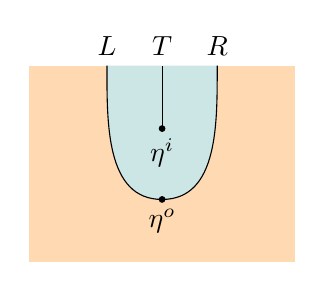
\begin{tikzpicture}
            \def\xright{0.7};
            \def\xleft{-\xright};
            \def\xmid{0};

            \def \ybot{0};
            \def \ymid{0.8};
            \def \yup{1.7};
            \def \ytop{2.5};

            \node [above] at (\xleft, \ytop) {$L$};
            \node [above] at (\xmid, \ytop) {$T$};
            \node [above] at (\xright, \ytop) {$R$};

            \filldraw[fill=orange!30, draw=white] (\xleft-1, \ytop) rectangle (\xright+1, \ybot);

            \draw [fill=blue!50!green!20] (\xleft, \ytop) to [out=-90, in=180] (\xmid, \ymid) to [out=0, in=-90] (\xright, \ytop);

            \filldraw[black] (\xmid, \ymid) circle (1 pt);
            \node [below] at (\xmid, \ymid) {$\eta^o$};
            \filldraw[black] (\xmid, \yup) circle (1 pt);
            \node [below] at (\xmid, \yup) {$\eta^i$};
            \draw (\xmid, \yup) -- (\xmid,\ytop);

        \end{tikzpicture}
    \]
    它是用$R \circ \eta^i \circ L$扩展的内层单元和外层单元$\eta^o$的垂直组合。其成分为:
    \[ \eta_a = R(\eta^i_{L a}) \circ \eta^o_a\]

    组合单子的乘法是一个自然变换:
    \[ \mu \colon R \circ T \circ L \circ R \circ T \circ L \to R \circ T \circ L \]
    它由如下字符串图给出:

    \[
        \begin{tikzpicture}
            \def \xmid          {0};
            \def \xr               {0.3};
            \def \xrt             {0.9};
            \def \xrr             {1.5}
            \def \xrm            {0.6}
            \def \xrightmost {2}
            \def \xl {-\xr}
            \def \xlt {-\xrt}
            \def \xll {-\xrr}
            \def \xlm {-\xrm}
            \def \xleftmost {-\xrightmost}

            \def \ybot           {0};
            \def \ymidbot     {0.2};
            \def \yeps          {0.8};
            \def \ymu           {1.5}; % mu
            \def \ymid          {1.9};
            \def \ymidtop     {2.6}
            \def \ytop           {2.7};
            \def \ylabel        {\ytop - 0.3};
% functors
            \node [above] at (\xlm, \ytop)  {$L$};
            \node [above] at (\xmid, \ytop)  {$T$};
            \node [above] at (\xrm, \ytop) {$R$};

            \node [below] at (\xll, \ybot) {$L$};
            \node [below] at (\xlt, \ybot) {$T$};
            \node [below] at (\xl, \ybot) {$R$};
            \node [below] at (\xr, \ybot) {$L$};
            \node [below] at (\xrt, \ybot) {$T$};
            \def\xrightmost{2}
        \end{tikzpicture}
    \]
    这是由外层辅元$\varepsilon^o$扩展的乘法$\mu^i$的垂直组合。其成分为:
    \[ \mu_c = R(\mu^i_{L c}) \circ (R \circ T) (\varepsilon^o_{(T\circ L)c})\]

    \subsection{State monad transformer(状态单子变换器)}

    让我们展开这些方程式,看看状态单子变换器的情况。状态单子是由柯里化伴随(currying adjunction)生成的。左函子$L_s$是乘积函子\hask{(a, s)},右函子$R_s$是指数(exponential),也称为读者函子(reader functor)\hask{(s -> a)}。

    正如我们之前看到的,外层辅元$\varepsilon^o_a$是函数应用:
    \begin{haskell}
        counit :: (s -> a, s) -> a
        counit (f, x) = f x
    \end{haskell}
    单元$\eta^o_a$是柯里化的对偶构造函数:
    \begin{haskell}
        unit :: a -> s -> (a, s)
        unit x = \s -> (x, s)
    \end{haskell}

    我们将保持内层单子$(T, \eta^i, \mu^i)$的任意性。在Haskell中,我们将此三元组称为\hask{m},\hask{return}和\hask{join}。

    通过应用状态单子变换器到单子$T$,我们得到的组合单子是$R \circ T \circ L$,或者在Haskell中:
    \begin{haskell}
        newtype StateT s m a = StateT (s -> m (a, s))
    \end{haskell}

    \begin{haskell}
        runStateT :: StateT s m a -> s -> m (a, s)
        runStateT (StateT h) s = h s
    \end{haskell}

    单子变换器的单元是$\eta^o$和$R \circ \eta^i \circ L$的垂直组合。其成分为:
    \[ \eta_a = R(\eta^i_{L a}) \circ \eta^o_a \]

    在这个公式中有许多部分,因此我们逐步分析它。我们从右边开始:我们有伴随单元的$a$成分,它是从$a$到$R (L a)$的箭头。在Haskell中,它是函数\hask{unit}。
    \begin{haskell}
        unit :: a -> s -> (a, s)
    \end{haskell}
    让我们在某个\hask{x :: a}上评估此函数。结果是另一个函数\hask{s -> (a, s)}。我们将此函数作为参数传递给$R(\eta^i_{L a})$。

    $\eta^i_{L a}$是\hask{return}的内层单子的成分,取自$L a$。在这里,$L a$的类型是\hask{(a, s)}。所以我们将多态函数\hask{return :: a -> m a}实例化为函数\hask{(a, s) -> m (a, s)}。(类型推断器将自动为我们执行此操作。)

    接下来,我们使用$R$提升\hask{return}的这个成分。在这里,$R$是指数$(-)^s$,因此它通过后组合(post-composition)提升一个函数。它将\hask{return}后组合到传递给它的任何函数上。在我们的例子中,那是由\hask{unit}生成的函数。注意类型是匹配的:我们在\hask{s -> (a, s)}之后进行后组合\hask{(a, s) -> m (a, s)}。

    我们可以将此组合的结果写为:
    \begin{haskell}
        return x = StateT (return . \s -> (x, s))
    \end{haskell}
    或者,内联函数组合:
    \begin{haskell}
        return x = StateT (\s -> return (x, s))
    \end{haskell}
    我们插入了数据构造函数\hask{StateT}以使类型检查器满意。这是复合单子的\hask{return},用内层单子的\hask{return}表示。

    相同的推理可以应用于某个$a$的复合$\mu$的公式:

    \[ \mu_a = R(\mu^i_{L a}) \circ (R \circ T) (\varepsilon^o_{(T\circ L) a})\]
    内层$\mu^i$是单子\hask{m}的\hask{join}。应用$R$将其转化为后组合。

    外层$\varepsilon^o$是在$T(L a)$上应用的函数或\hask{m (a, s)}。它是一个类型为:
    \begin{haskell}
        (s -> m (a, s), s) -> m (a, s)
    \end{haskell}
    的函数,通过插入适当的数据构造函数,可以将其写为\hask{uncurry runStateT}:
    \begin{haskell}
        uncurry runStateT :: (StateT s m a, s) -> m (a, s)
    \end{haskell}
    $(R \circ T)$的应用通过$R$和$T$的函子组合提升了此$\varepsilon$的成分。前者是通过后组合实现的,后者是单子\hask{m}的\hask{fmap}。

    将所有这些结合在一起,我们得到状态单子变换器的\hask{join}的无点公式:
    \begin{haskell}
        join :: StateT s m (StateT s m a) -> StateT s m a
        join mma = StateT (join . fmap (uncurry runStateT) . runStateT mma)
    \end{haskell}
    在这里,部分应用的\hask{(runStateT mma)}从参数\hask{mma}中剥离了数据构造函数:
    \begin{haskell}
        runStateT mma :: s -> m (a, x)
    \end{haskell}

    我们之前的\hask{MaybeState}示例现在可以使用单子变换器重写为:
    \begin{haskell}
        type MaybeState s a = StateT s Maybe a
    \end{haskell}

    可以通过将\hask{StateT}单子变换器应用于恒等函子(identity functor)来恢复普通的\hask{State}单子,恒等函子在库中定义了一个\hask{Monad}实例(注意,在此定义中跳过了最后一个类型变量\hask{a}):
    \begin{haskell}
        type State s = StateT s Identity
    \end{haskell}

    其他单子变换器遵循相同的模式。它们定义在单子变换器库\hask{MTL}中。

\end{document}